\documentclass{report}
\usepackage[T1]{fontenc}
\usepackage{parskip}
\usepackage{graphicx}
\usepackage{fancyvrb}
\usepackage{hyperref}

\graphicspath{{./images/}}
\begin{document}
	\chapter{Introduction}
	This first chapter, we will breeze through the topics of Angular, componentization, single page web app and others that we will delve into in detail in rest of the book.
	
	\section{Just what is Angular?}
Angular is a framework for programming the web using components. The web componentization movement started a little while ago. Now, there are many serious players in this field, e.g., Angular, React, Svelte, Vue, just to name a few. The native web technologies (HTML, CSS, and JavaScript) have also started out in this direction by introducing the Web Components \href{https://www.webcomponents.org/specs}{specification}.

All these different libraries and frameworks have about the same concept of what constitutes a component. For example, an Angular component has all the necessary ingredients to make a chunk of HTML look and behave in a specific way wherever it's used. That's right! An Angular component can be tucked anywhere in a web page and still afford to look and behave consistently. That's pure reusability for you! How does it achieve that? An Angular component has all the required HTML, CSS, and JavaScript tightly encapsulated and is thus able to bring reusability to the table. Before diving into the details, let's get to see an Angular component in action!

Let's start by installing Node.js and the required NPM packages. I suggest using a node version manager like \href{https://github.com/jasongin/nvs}{NVS} to manage installations of different Node versions on your machine.

Install Node.js version 16.17+. Ensure that the version of NPM is 8.19+ and the browser is Chrome, version 100+.

When learning and working with Angular, \textsl{Angular CLI} is our best friend. \textsl{CLI} stands for \textsl{Command Line Interpreter}. We need to type in various commands on the command line to use the features of CLI, like e.g., creating a new Angular project, adding components to an existing one, etc. Each of these tasks involve writing some boiler-plate code which the CLI takes care. The CLI, thus makes it easy to work with Angular projects.

First, let's start by installing CLI using the command line\footnote{The version being installed here is 16.1.0. However, this command should also upgrade an older version of CLI if one's installed.}:

\texttt{npm install -g @angular/cli@16.1.0}

Next, let's create an Angular project using the newly installed CLI. The name of the project is \textsl{booklibrary}. Ensure there's no folder by that name and in the command line enter: 

\texttt{ng new booklibrary --prefix bk --defaults --standalone}

We have invoked the \verb|new| command of the CLI that takes care of creating an Angular project! After a few moments of entering those seemingly magic incantations, if everything goes well, we should be greeted by the message: 'Successfully initialized git.' and should see a new folder with the name \textsl{booklibrary} created. We are good to go! \verb|cd| into the folder and enter:

\texttt{ng serve}

After a few moments, We should see the message: \textbf{\texttt{Angular Live Development Server is listening on localhost:4200}}. Open \url{http://localhost:4200} in a browser and, lo! we should see our very first web app up and running!

What magic did the CLI perform to bring up the web app? Let's investigate starting from the \textsl{booklibrary} folder that was created by the \verb|ng new| command! There should be files in that folder as shown in the figure below:

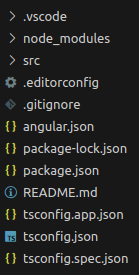
\includegraphics[scale=0.5]{project-structure}

These files were created by the \verb|ng new| command and constitute the Angular project. Among the files there's a \textsl{package.json} file that defines the \textsl{npm packages} that the project depends on. The important dependencies are:

\begin{itemize}
	\item @angular packages, the main libraries that constitute the Angular framework.
	\item rxjs - a library that makes it convenient to work with Observables.
	\item zone.js - a library for change detection; a core function required by Angular framework.
	\item dependencies for developing the application like Angular CLI, Typescript compiler, Jasmine unit testing tool, etc.
\end{itemize}

Other files of interest in the project are
\begin{itemize}
	\item \textsl{angular.json}. Angular specific project settings are stored here.
	\item The Typescript compiler has its own configuration files in the project folder named \textsl{tsconfig.json} and \textsl{tsconfig.app.json}. They store options required by the Typescript compiler, like e.g., an option for generating source maps\footnote{Source maps allow us to debug our app in the browser's dev console with the original Typescript source code!}.
\end{itemize}

Enough of seeing the project structure, now, let's delve into the code!

\section{Our First Angular Component}
All the component code resides in the \textsl{src/app} folder. The CLI has created our first Angular component in that folder. The component is named \textsl{AppComponent} and consists of four files:

\begin{itemize}
	\item app.component.ts - Defines the behavior (functionality) of the component in TypeScript language.
	\item app.component.spec.ts - Contains Unit tests for the component's functionality coded in TypeScript.
	\item app.component.html - Defines the content structure in terms of HTML elements contained in the component.
	\item app.component.css - Defines how the component looks by way of CSS style rules.
\end{itemize}

Looking at \textsl{app.component.ts} we see the following TypeScript code:
\begin{Verbatim}[numbers=left]
import { Component } from '@angular/core';
import { CommonModule } from '@angular/common';

@Component({
  selector: 'bk-root',
  standalone: true,
  imports: [CommonModule],
  templateUrl: './app.component.html',
  styleUrls: ['./app.component.css']
})
export class AppComponent {
  title = 'booklibrary';
}
\end{Verbatim}

Holy Cow! The app itself is a component! This fact is being made known by the use of the \verb|@Component()| decorator. A \textsl{decorator} is so called because of its ability to give additional meaning to, i.e. \textsl{decorate}, TypeScript language elements. Here we use the \verb|@Component| decorator to convey that the \verb|AppComponent| is an Angular component and not just a \textsl{regular} TypeScript class. As we will see in detail further, what makes an Angular component special is that it has an associated view defined in terms of HTML which says what will be displayed when the component is visible in a web page. In the above example, the view (HTML) is in a separate file, \verb|app.component.html|. This fact is made known by the \verb|templateUrl| key (line 8) of the configuration object that's the argument to \verb|@Component()| decorator which is being \textsl{called} like a function. We also define how the component looks by specifying the CSS style rules in a file whose path is specified in the \verb|styleUrls| key of the same configuration object argument.

How do we see our component at work in a web page? To create the component in a web page, we use custom tags as given by the \verb|selector| key of the \verb|@Component()| decorator of \verb|AppComponent|. The custom tags create custom elements whose HTML content is specified by the file pointed to by the \verb|templateUrl| and whose appearance is defined by the CSS in file(s) given by \verb|styleUrls| of the \verb|@Component()|. Thus, the custom tag \verb|bk-root| is used in \verb|index.html| file of src folder to create the AppComponent element.

\section{Naming conventions}
Angular CLI names component classes with names ending with \verb|Component|. The classes are defined in files whose names end with \verb|component.ts|. To avoid name clashes, names of custom tags created by Angular are prefixed with some combination of letters. The \verb|--prefix bk| that we used in the \verb|ng new| command specifies that throughout the application, Angular must prefix custom tags with the letters \verb|bk|.

The \verb|imports| key of \verb|@Component()| decorator specifies that Angular must look into its CommonModule for components, directives, pipes and other functionality that's referred to in the template of the component. This is how we can reuse functionality implemented elsewhere. For example, if we have used a custom tag \verb|bk-books-collected| which is defined in the BooksCollected component decorator, we need to include this component in the list of \verb|imports|.

The \verb|standalone| key of \verb|@Component()| decorator specifies that the component doesn't belong to any specific module.

\section{Bootstrapping the application}
Angular CLI automatically generates the required logic to start the app in a file called \verb|main.ts|, inside the \verb|src| folder.

\begin{Verbatim}[numbers=left]
import { bootstrapApplication } from '@angular/platform-browser';
import { appConfig } from './app/app.config';
import { AppComponent } from './app/app.component';
bootstrapApplication(AppComponent, appConfig)
  .catch((err) => console.error(err));
\end{Verbatim}

But, the script needs to run from a web page right? Yes, right! The \verb|index.html| file in \verb|src| folder is the web page that represents the App. How can we be so sure? The \verb|bk-root| custom tag in the file creates an instance of AppComponent.

\fvset{numbers=left, frame=topline, framesep=5mm}

\chapter{Templating}
In this chapter we will learn how to make our components display dynamic content on a web page. This way, e.g., we can greet our library members by their name whenever they log in to our application!

\section{Interpolation}
For the purpose of explaining the concept, we will resort to using inline templates in our components. We need to replace the \verb|templateUrl| with \verb|template| key in our \verb|@Component| decorator as shown below.
 
\begin{Verbatim}[label=v2.1.0]
import { Component } from '@angular/core';

@Component({
  selector: 'bk-root',
  standalone: true,
  template: "<h2>Welcome to Greenie's Book Library</h2>",
})
export class AppComponent {
}
\end{Verbatim}

Two things to note from the example above:
\begin{itemize}
\item We are not importing \verb|CommonModule| anymore as we are not using any components, directives or pipes from the \verb|CommonModule| in our simple example.
\item We are using inline template and kept the HTML content of our component in the \verb|template| key of \verb|@Component()| decorator. The template is a string of HTML code demarced with the double quotes. We could have used single quotes to demarc the code but would have encountered a problem as there's a single quote as part of the HTML code (\textsl{Greenie's}).
\end{itemize}

After the above code changes we must be able to see a welcome message: Welcome to Greenie's Book Library!

Now, let's spruce up the greeting message a bit by including the name of the library member dynamically. As of now, we will not fetch the name from the server as that will involve some more technical wizardry. Let's modify the previous code to make the greeting a little more personalised:

\begin{Verbatim}[label=v2.1.1]
import { Component } from '@angular/core';

@Component({
  selector: 'bk-root',
  standalone: true,
  template: "<h1>Hi {{ user.name }}!</h1><h2>Welcome to Greenie's Book Library</h2>",
})
export class AppComponent {
  user = { name: 'Hari' };
}
\end{Verbatim}

We have used what's called as \textsl{interpolation} to display the user's name which is set in the component! How does this work? In summary, the technique allows us to evaluate any TypeScript expression and include the result as part of the template. Anything in the template that's enclosed in double braces \verb|{{}}| will be treated as a TypeScript expression and evaluated in the context of the component. Thus the expression can refer to various properties of the component. In the above example, the expression \verb|{{ user.name }}| refers to the user property of AppComponent whose name key is evaluated.

Another thing Angular does for us is that the expression is evaluated everytime the involved properties change their values and the view (DOM) is updated to reflect the changes! Angular also saves us from having to debug in situations where we may be referring to properties that don't actually exist in the component. For example, if we have erroneously referred to the property \verb|user| by the name \verb|users| in the TypeScript expression like so: \verb|{{ users.name }}|, the compiler stops us in the tracks by throwing a compile-time error: \texttt{Property 'users' does not exist on type 'AppComponent'. Did you mean 'user'?} The compiler even goes so far as to suggest what we may have meant to use!

Another feature of Angular is for references to properties that are not initialized, having the value \verb|undefined| or \verb|null|, Angular uses the empty string instead of \verb|undefined| or \verb|null|. However, if we are referring to a key of the property as in the example above, the compile step fails with the message: \texttt{Object is possibly 'undefined'}. This is a good thing that allows us to catch errors early. Had the compiler not stopped us from going ahead, we would have been confused as to why we are not seeing the expected result after running the app. To see the compiler catching us in the act, we need to modify the code a bit:

\begin{Verbatim}[label=v2.1.1a]
import { Component } from '@angular/core';

@Component({
  selector: 'bk-root',
  standalone: true,
  template: "<h1>Hi {{ user.name }}!</h1><h2>Welcome to Greenie's Book Library</h2>",
})
export class AppComponent {
  user: { name: string } | undefined;
}
\end{Verbatim}

You may feel that the example is too contrived and will not occur in the wild. But, when we are getting the user details from a server, the scenario is very much plausible and the above code is how we would handle it. The way to resolve the compiler error, we need to use the optional chaining operator \verb|?.| instead of the property access operator \verb|.|. The code now becomes:

\begin{Verbatim}[label=v2.1.2]
import { Component } from '@angular/core';

@Component({
  selector: 'bk-root',
  standalone: true,
  template: "<h1>Hi {{ user?.name }}!</h1><h2>Welcome to Greenie's Book Library</h2>",
  styleUrls: ['./app.component.css'],
})
export class AppComponent {
  user: { name: string } | undefined;
}
\end{Verbatim}

But, we won't be seeing any user's name displayed now as the user property is not initialized (and hence would be having the value \verb|undefined|). The above code is how we would handle a scenario where the user property is set from an API call to a server.

\section{Property Binding}
Interpolation is just one specialized application of a central feature of Angular known as property binding. To understand what this feature is all about we must remember that the Angular framework helps us in creating and working with DOM nodes that can contain custom content, can be styled independently and made to exhibit certain behavior. The property binding feature helps to support this vision by making it possible to set \emph{any} property of a DOM node, using a similarly named attribute on the HTML tag that creates the DOM node. The value of the attribute is treated as a TypeScript expression and evaluated before being assigned to the property mirrored by the attribute. Since, this is an Angular feature and not something natively provided by HTML we use special syntax that triggers it. We enclose the attribute in square brackets. This Angular specific syntax is not valid HTML and is allowed only inside a component's template. Angular parses a component's template and turns it into valid HTML plus TypeScript code that acheives the property binding. The previously shown interpolation technique can be rewritten using the property binding technique as shown below.

\begin{Verbatim}[label=v2.1.3]
import { Component } from '@angular/core';

@Component({
  selector: 'bk-root',
  standalone: true,
  template: `<h1 [textContent]="'Hi ' + user?.name + '!'"></h1>
  <h2>Welcome to Greenie's Book Library</h2>`,
})
export class AppComponent {
  user: { name: string } | undefined;
}
\end{Verbatim}

Note that I have used a pair of backticks \verb|`| for enclosing the template string. Using backticks allows me to break up the string onto multiple lines. But, what's really of interest in the code example above is the use of property binding technique to bind the DOM property \verb|textContent| to the attribute \verb|textContent|'s value. When we run the app, we see the h1 tag display \texttt{Hi null!} message. Previously, Angular was not displaying \verb|null| or \verb|undefined| when we were using the interpolation syntax. With the property binding there are no such safety valves. Hence, interpolation is more appropriate when we just want to display the value of a component's property where property binding is more awkward to use and requires more code to be written (\verb|[textContent]=".."|).

As in the case of interpolation, property binding binds the DOM property to the attribute's value as specified in the template. The value is evaluated as a TypeScript expression. Hence, whenever the value of the TypeScript expression changes, the DOM property is updated to the new value. How does the above example work? Why setting the \verb|textContent| attribute using Angular's special property binding syntax is able to achieve the behavior we see above? It may be known that \verb|textContent| is a \href{https://developer.mozilla.org/en-US/docs/Web/API/Node/textContent}{property} of every DOM node. Setting that property replaces all the child DOM nodes with a single text node. And, that's what we have done here. We have used Angular's special property binding syntax to set that  \verb|textContent| property via a similarly named attribute. In fact, any DOM node's property, like e.g., the \verb|hidden| property or an \verb|input| element's \verb|value| property, can be set in this way. The Angular parser that parses the special property binding syntax is case insensitive - the attribute enclosed in square brackets must exactly match the name of the DOM property even in terms of the casing. Thus, in the previous example the attribute must be specified as \verb|[textContent]| and not \verb|[textcontent]| or \verb|[TEXTCONTENT]|.

To make use of the full power of the property binding technique, we usually have a reference to some property of the template's component in the expression value of the DOM property, like \verb|user|, in the previous example. When the value of the component's property changes, the template's DOM property gets updated. In the previous example, whenever the value of \verb|user| or \verb|user.name| property changes, the text content of the \verb|h1| element is updated to reflect the changed value. At this point, I know your mind must be racing to see a demo of this changing of the property's value updating the DOM. As noted in the section on interpolation, this feature of Angular is called change detection. To see it in action we need a way to change the component's property in real time, like e.g., in response to a button click event.

\section{Reacting to DOM events}
The component's template in the code below shows a button tag with a handler for DOM click events.

\begin{Verbatim}[label=v2.1.4]
import { Component } from '@angular/core';

@Component({
  selector: 'bk-root',
  standalone: true,
  template: `<h1 [textContent]="'Hi, ' + user.name + '!'"></h1>
  <h2>Welcome to Greenie's Book Library</h2>
  <button (click)="turnGreen()">Turn me green!</button>`,
})
export class AppComponent {
  user = { name: "Mr. Red" };

  turnGreen() {
    this.user.name = "Mr. Green";
  }
}
\end{Verbatim}

Angular makes it easy to handle \href{https://developer.mozilla.org/en-US/docs/Web/Events#event_listing}{DOM events} by allowing us to specify in the template of a component the TypeScript code that should execute in response to an event. Again, as you may guess, there's special syntax to do this. The Angular parser looks for special attributes on HTML tags in the template of a component. These attributes are special in that they are not standard HTML attributes. They are enclosed within parantheses and are named after the name of a DOM event, e.g., \verb|(click)| or \verb|(keydown)|. The value of the attribute is evaluated as TypeScript code that gets executed in the context of the component's class when the event occurs. Note that just like regular HTML attribute values the code must be enclosed in double quotes. In the component template above, you can identify the code \verb|turnGreen()| inside the double quotes as a method call. The method is defined in the component's class. Inside the method definition, we have code to change the user's name to "\texttt{Mr. Green}". The method is called when the user clicks on the button.

\section{Composition}
It's possible to compose an Angular component using other Angular components. After all, the whole idea of developing components in the first place is to be able to use them as part of other complex components. From the point of JavaScript it has always been possible to compose a class or object with other classes and objects. But, how do we compose a HTML element with other HTML elements? We have already seen the answer to this problem in chapter 1. We just use the proper custom tag (given by the selector key of the \verb|@Component| decorator) in the template of another component. In the example above, suppose we want to show

\end{document}
